\chapter{Experimentación}\label{cap:experimentacion}

El objetivo de estos experimentos es analizar el rendimiento de la aplicación móvil ALERTAR en términos de almacenamiento, transmisión de datos, tiempos de operación y conectividad entre dispositivos. Para lograrlo, se realizaron mediciones y comparaciones entre el espacio requerido y el espacio real que ocupan los datos, junto con los tiempos de transmisión de estos.

El dispositivo utilizado como borde es un \textit{Samsung Galaxy Tab A7 Lite} con un procesador \textit{Qualcomm Snapdragon 662} de \textit{2.0 GHz} con 8 núcleos, \textit{4 GiB} de memoria principal y sistema operativo \textit{Android 11}. El dispositivo utilizado como niebla es un \textit{Pixel 8} con procesador \textit{Google Tensor G3} con 9 núcleos (uno de \textit{2.9 GHz}, cuatro de \textit{2.4GHz} y cuatro de \textit{1.7 GHz}), \textit{8 GiB} de memoria principal y sistema operativo \textit{Android 15}. La nube cuenta con un procesador Intel Xeon CPU E5-2630 de \textit{2.3 GHz} y \textit{16 GB} de memoria principal y sistema operativo \textit{Linux}. Los dispositivos de borde y niebla se conectaron mediante una red inalámbrica de área local con un ancho de banda de entre \textit{85 mbps} y \textit{100 mbps}.

En la sección \ref{sec:datosUtilesVSalmacenamiento} se llevó a cabo una evaluación del espacio de almacenamiento requerido respecto del espacio real que ocupan los datos. En la sección \ref{sec:datosUtilesVsDatosEnTransito} se comparan los datos útiles contra los datos en tránsito para detectar sobrecargas de información. En la sección \ref{sec:tiemposDeLasOps} se desarrolla una evaluación del rendimiento de la aplicación considerando los tiempos de procesamiento individuales en los dispositivos de borde y los tiempos de procesamiento externos necesarios para recibir una respuesta desde la nube u otro dispositivo de niebla. Finalmente, en la sección \ref{sec:conectividadDispositivos} se realizó una prueba de estrés en los dispositivos de niebla para evaluar su capacidad de soportar múltiples conexiones simultáneas a través de una red de área local desde los dispositivos de borde.



\section{Datos útiles contra espacio de almacenamiento}
\label{sec:datosUtilesVSalmacenamiento}
Este experimento busca comprender la diferencia entre el tamaño requerido y real de los datos para identificar e intentar reducir la sobrecarga innecesaria a fin de, a futuro, poder optimizar el almacenamiento y mejorar el rendimiento de la aplicación. Para realizarlo se seleccionó la tabla de datos Paciente, que contiene la información personal de cada paciente y es una de las tablas con más parámetros en el sistema, lo que la convierte en un caso altamente significativo. A continuación se enumeran las consideraciones y pasos realizados para realizar la medición:
\begin{enumerate}
    \item Se calculó el tamaño requerido para cada tipo de dato. Las mediciones se detallan en la Tabla \ref{tabla:TamReqSegTipoDat} donde en la primera columna se muestra el nombre del atributo, en la segunda columna se indica el tipo de dato del atributo, y en la tercera columna se presenta el valor asignado a cada atributo. Cabe destacar que, en la tercera columna, algunas casillas están en blanco porque corresponden a tipos de datos enteros, cuyo tamaño será el mismo independientemente del valor utilizado. Se consideró que un entero ocupa 4 bytes y que cada carácter ocupa 1 byte en la base de datos. En la última columna se especifica el tamaño requerido para cada atributo en función del tipo de dato y el valor asignado. 
    
    \item A fin de analizar el impacto que tiene la inserción de diferentes tipos de registros, se insertaron registros de tipo \textit{Cama}. De esta manera, se insertaron 4000 registros de tipo \textit{Paciente}, donde cada registro requiere 136 bytes de datos útiles y 2000 registros de tipo \textit{Cama}, donde cada registro requiere 44 bytes de datos útiles. Así, al finalizar el experimento se contó con 6000 registros. 
    
    \item Se determinó el tamaño total requerido por registro. Esto se realizó comenzando con un grupo de cien registros y luego incrementando de cien en cien hasta alcanzar un total de 6000 registros. Las mediciones se hicieron cada cien registros insertados. Primero se insertaron los registros de tipo \textit{Paciente} y luego los de tipo \textit{Cama}. La base de datos inicialmente se encontraba vacía.
    
    \item Se calculó la ``sobrecarga'' que representa la diferencia porcentual entre el tamaño requerido de los registros y el tamaño final que ocupan en la base de datos. Los resultados de estas mediciones se encuentran en las Tablas \ref{tabla:TamReqYRealConOverPacientes}\ref{tabla:TamReqYRealConOverCamas}.
\end{enumerate}

%Primero, se calculó el tamaño requerido para cada tipo de dato, como se muestra en la Tabla \ref{tabla:TamReqSegTipoDat}. Para esto, se consideró que un entero ocupa 4 bytes y cada carácter ocupa 1 byte en la base de datos.

%Después de calcular el tamaño requerido por tipo de dato, se determinó el tamaño total requerido por registro. Esto se realizó comenzando con un grupo de cien registros y luego incrementando de cien en cien hasta alcanzar un total de 6000 registros.

%En tercer lugar se insertó dicha cantidad de registros en la base de datos y se midió cada cien inserciones el tamaño de la base de datos, la cual, inicialmente, se encuentra vacía. 

%Por último, se calculó la ``sobrecarga'' la cual representa la diferencia porcentual entre el tamaño requerido de los registros y el tamaño final que ocupan en la base de datos Tablas \ref{tabla:TamReqYRealConOverPacientes}\ref{tabla:TamReqYRealConOverCamas}.



En la Figura \ref{fig:DatosUtilesVsEspacio2} se muestra la sobrecarga de espacio utilizado para el almacenamiento secundario sobre las diferentes cantidades de registros. Las barras azules se corresponden con la tabla Paciente y las rojas con la tabla Cama. Se puede observar una mayor eficiencia (menor sobrecarga) a medida que el número de registros aumenta. Esto significa que, conforme se agreguen más registros, el espacio de almacenamiento será mejor aprovechado. Sin embargo, al comenzar a insertar datos a una tabla diferente, se produce un decremento significativo de la eficiencia (a partir de los 4100 registros), pasando de 70\% a 415\% de sobrecarga. Luego, la sobrecarga disminuye y, por lo tanto, la eficiencia aumenta.

Finalmente se concluye que el aprovechamiento del almacenamiento mejora con el crecimiento de los registros dentro de una misma tabla, lo que indica un uso más efectivo del espacio conforme se van ingresando datos. Sin embargo, la introducción de datos de diferentes tablas o tipos de datos provoca un aumento en la sobrecarga.
\begin{table}[]

\centering
\captionof{table}{Tamaño requerido según tipo de dato}
\label{tabla:TamReqSegTipoDat}
\begin{tabular}{|l|l|c|c|}
\hline
\textbf{Atributo} & \textbf{Tipo de dato} & \textbf{Valor utilizado} & \textbf{Tamaño requerido (bytes)} \\ \hline
sync\_id & integer & & 4 \\ \hline
domain & string & ``/hosp00/sector00'' & 16 \\ \hline
pacienteId & integer & & 4 \\ \hline
numeroHC & string & ``P0000000001'' & 11 \\ \hline
fechaIngreso & integer & & 4 \\ \hline
numeroDocumento & string & \textit{(8 dígitos ASCII)} & 8 \\ \hline
tipoDocumento & string & ``DNI'' & 3 \\ \hline
idPaisExpedicion & string & ``.ar'' & 3 \\ \hline
nombres & string & ``Francisco'' & 9 \\ \hline
apellidos & string & ``Repetto'' & 7 \\ \hline
sexo & string & ``M'' & 1 \\ \hline
calle & string & ``Av.Argentina'' & 12 \\ \hline
numero & string & ``100'' & 3 \\ \hline
piso & string & ``-'' & 1 \\ \hline
idProvincia & integer & & 4 \\ \hline
idLocalidad & integer & & 4 \\ \hline
CP & string & ``8300'' & 4 \\ \hline
telefono & string & ``2995000000'' & 10 \\ \hline
telefonoFamiliar1 & string & ``2995111111'' & 10 \\ \hline
telefonoFamiliar2 & string & ``2995222222'' & 10 \\ \hline
fechaNacimiento & integer & & 4 \\ \hline
deleted & integer & & 4 \\ \hline
\multicolumn{3}{|c|}{\textbf{TOTAL}} & \textbf{136} \\ \hline
\end{tabular}

\end{table}



%\begin{figure}
%    \centering
%    \includegraphics[width=\textwidth]{Imagenes/Experimentos/Diferencia entre datos útiles contra el espacio utilizado 1.pdf}
%    \caption{Diferencia entre datos útiles contra el espacio utilizado}
%    \label{fig:DatosUtilesVsEspacio1}
%\end{figure}

\begin{figure}
    \centering
    \includegraphics[width=\textwidth]{Imagenes/Experimentos/Diferencia entre datos útiles contra el espacio utilizado 2.pdf}
    \caption{Diferencia entre datos útiles contra el espacio utilizado}
    \label{fig:DatosUtilesVsEspacio2}
\end{figure}



\section{Datos útiles contra datos en tránsito}
\label{sec:datosUtilesVsDatosEnTransito}
El fin de este experimento es determinar la sobrecarga de información que se tiene a causa de la estructura y el formato requeridos por el protocolo de comunicación \textit{JSON}. Esto incluye elementos adicionales como etiquetas, delimitadores y otros metadatos necesarios para interpretar correctamente los datos enviados. 

Para este se utilizó un registro de tipo \textit{Paciente}, el cual se detalla en la Tabla \ref{tabla:TamReqSegTipoDat}. En las mediciones realizadas se observó que en tránsito hay 577 bytes lo cual significa una sobrecarga considerable de 441 bytes para transmitir un único registro con un tamaño de 136 bytes, produciendo una sobrecarga de 324\% al utilizar el formato \textit{JSON}.

Se puede afirmar que la eficiencia de transmisión es baja, ya que el tamaño real en tránsito es casi cuatro veces el tamaño necesario. Sin embargo, toda esta sobrecarga es a causa del formato estándar \textit{JSON}, el cual facilita la interoperabilidad entre sistemas diversos, brindando beneficios en cuanto uso, lectura, compatibilidad y flexibilidad de los datos. Aunque existe una sobrecarga a causa del formato, los beneficios mencionados justifican su uso.


%\begin{figure}
 %   \centering
 %   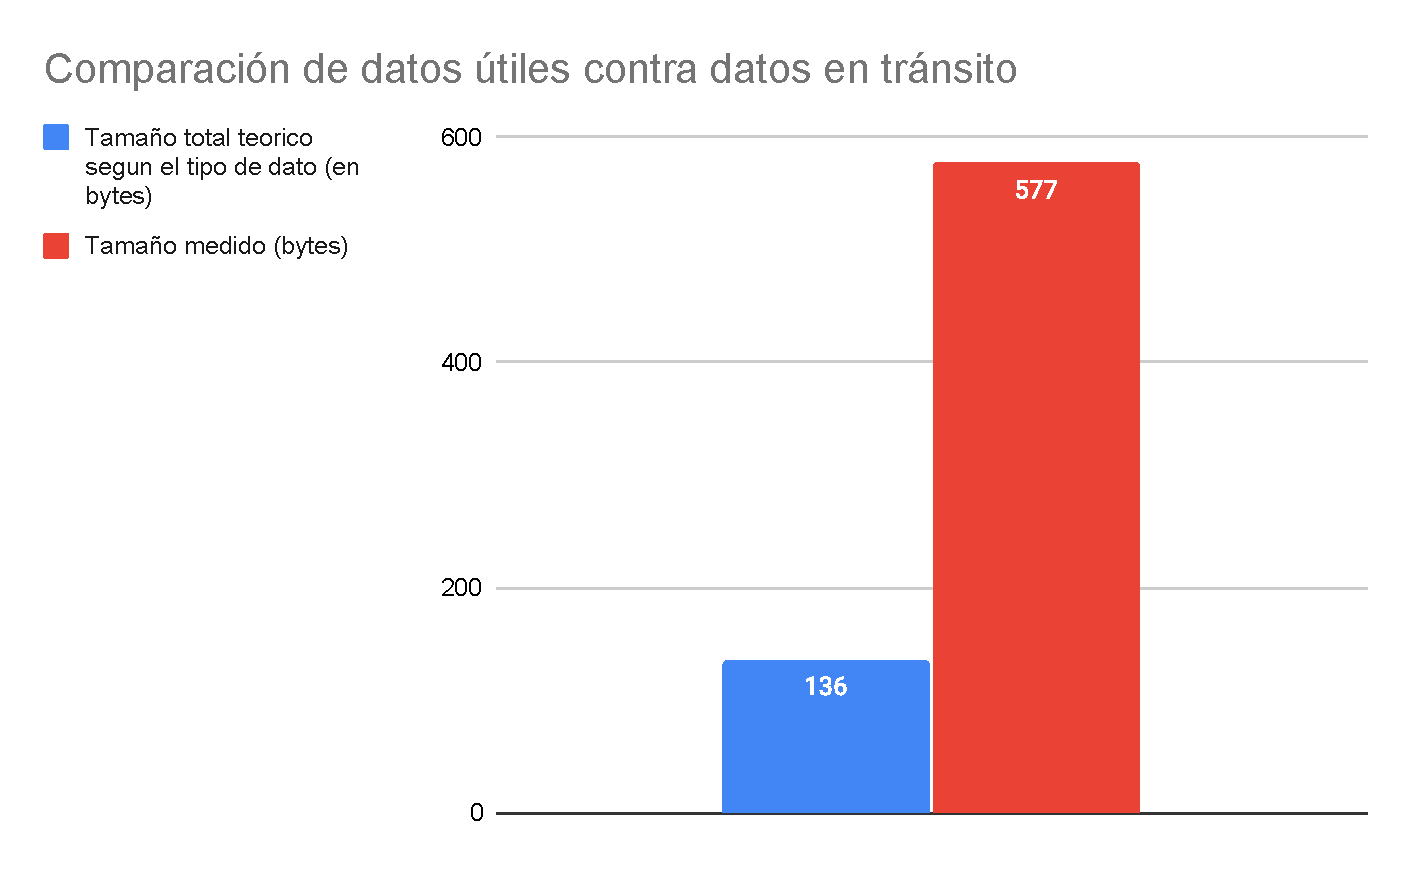
\includegraphics[width=\textwidth]{Imagenes/Experimentos/DatosUtilesVsDatosTransito.pdf}
 %   \caption{Tamaño total requerido y tamaño en tránsito}
 %   \label{fig:tamTotalvsTamTransito}
%\end{figure}
\section{Tiempos de las operaciones con diferentes tipos de conexión}
\label{sec:tiemposDeLasOps}
Este experimento se centra en evaluar y medir los tiempos de transmisión, procesamiento y el tiempo total en cada dispositivo, abarcando diversos casos de uso para las diferentes conexiones del sistema ALERTAR. El objetivo es determinar la eficiencia del sistema en completar operaciones críticas, identificar cuellos de botella donde el procesamiento puede ser excesivo, y evaluar el impacto de la latencia en las diferentes conexiones. El experimento consiste en ejecutar y medir casos de uso para los siguientes dos tipos de conexión:
\begin{itemize}
    \item \textbf{Dispositivo de borde $\leftrightarrow$ Nube: }El dispositivo de borde se encuentra conectado de manera directa a la nube. Además, existe un dispositivo de niebla a cargo del dominio al que está suscrito el de borde. Este dispositivo de niebla no participa de estas mediciones pero es necesario por requerimientos especificados en el protocolo de funcionamiento del sistema ALERTAR.
    \item \textbf{Dispositivo de borde $\leftrightarrow$ Dispositivo de niebla: }La conexión es por red de área local entre los dispositivos de borde y niebla.
\end{itemize}

Los casos de uso utilizados son los siguientes:
\begin{itemize}
    \item \textbf{Login: }Este caso de uso fue elegido debido a su complejidad en cuanto a requerimientos ya que implica hacer validaciones. En este, el dispositivo de borde envía un registro con sus datos para identificarse con el de niebla, el dispositivo de niebla se encarga de validar al usuario y como respuesta devuelve la información de los dominios a los que puede suscribirse el usuario.
    
    \item \textbf{DataSync: }Este caso de uso se eligió ya que es el encargado de sincronizar toda la información no actualizada en el dispositivo que acaba de iniciar sesión. A partir de este caso de uso se puede observar cómo se comporta el sistema a la hora de transmitir un volumen de información relativamente grande en comparación a operaciones más usuales como puede ser la inserción de un dato. Además de que permite observar cómo es el rendimiento de los dispositivos para procesar y almacenar dicha información en la base de datos.

    Durante la ejecución se hace una petición de sincronización desde el dispositivo de borde al dispositivo de niebla o nube, el de niebla o nube le envía toda la información actualizada al de borde (la cual consiste de 40 registros de tipo \textit{paciente} que implican 22073 bytes de almacenamiento), una vez recibida la información, el de borde la almacena en su base de datos local.

    En este experimento no se realiza ni mide el cambio de conexión ya que dicho procedimiento nunca se ejecuta. Esto se debe a que el dispositivo de borde se encuentra conectado a la nube por fuera de la red de área local o ya está conectado al dispositivo de niebla.
    \item \textbf{Insert: }Este caso de uso fue elegido a fin de evaluar como es el comportamiento de los dispositivos a la hora de insertar nuevos registros en el sistema ALERTAR. Para cada una de las pruebas se envía un nuevo registro, diferente a los ya ingresados pero con la misma cantidad de bytes, esto a causa de restricciones de integridad referencial de la base de datos. Una vez finalizado el procesamiento por parte del dispositivo de niebla o nube, este retorna un mensaje de completitud finalizando así el caso de uso y las mediciones.
\end{itemize}

Cada experimento se repitió diez veces. En la Figura \ref{fig:evaluacionInicial} se muestran los resultados de cada experimento, diferenciando los tiempos máximos y promedios obtenidos entre las 10 muestras. En el identificador de cada barra se distingue si la conexión del dispositivo de borde es con la nube (BN) o con el dispositivo de niebla (BDF).

En las operaciones \textit{Insert} y \textit{Login} se observa que casi todo el tiempo de ejecución es utilizado por las transmisiones y cómputo en el dispositivo de niebla, teniendo el dispositivo de borde una carga mínima, estos valores se consideran adecuados dado el dominio de la aplicación. 

Las operaciones de \textit{dataSync} son las que mayor tiempo total conllevan debido a que son las que transmiten y producen la inserción del mayor volumen de registros, produciendo una mayor carga de cómputo en los dispositivos de borde ya que deben realizar almacenamiento. En la conexión entre dispositivo de borde y nube se puede observar un menor tiempo externo que en la conexión borde con niebla. La nube cumple el rol de ``caché'' para devolver los registros a sincronizar al dispositivo de borde, por lo que en lugar de hacer una petición al dispositivo de niebla que contiene la copia primaria de los datos, la nube busca los datos directamente en su base de datos local. La diferencia en los tiempos de procesamiento externo se atribuye a las diferencias de \textit{hardware} y tipo de base de datos que posee la nube comparada a los dispositivos móviles. Se considera que los valores obtenidos son adecuados para el dominio de aplicación, tanto para el acceso de los registros en los dispositivos de niebla como para el almacenamiento en los dispositivos de borde.


\begin{figure}
    \centering 
        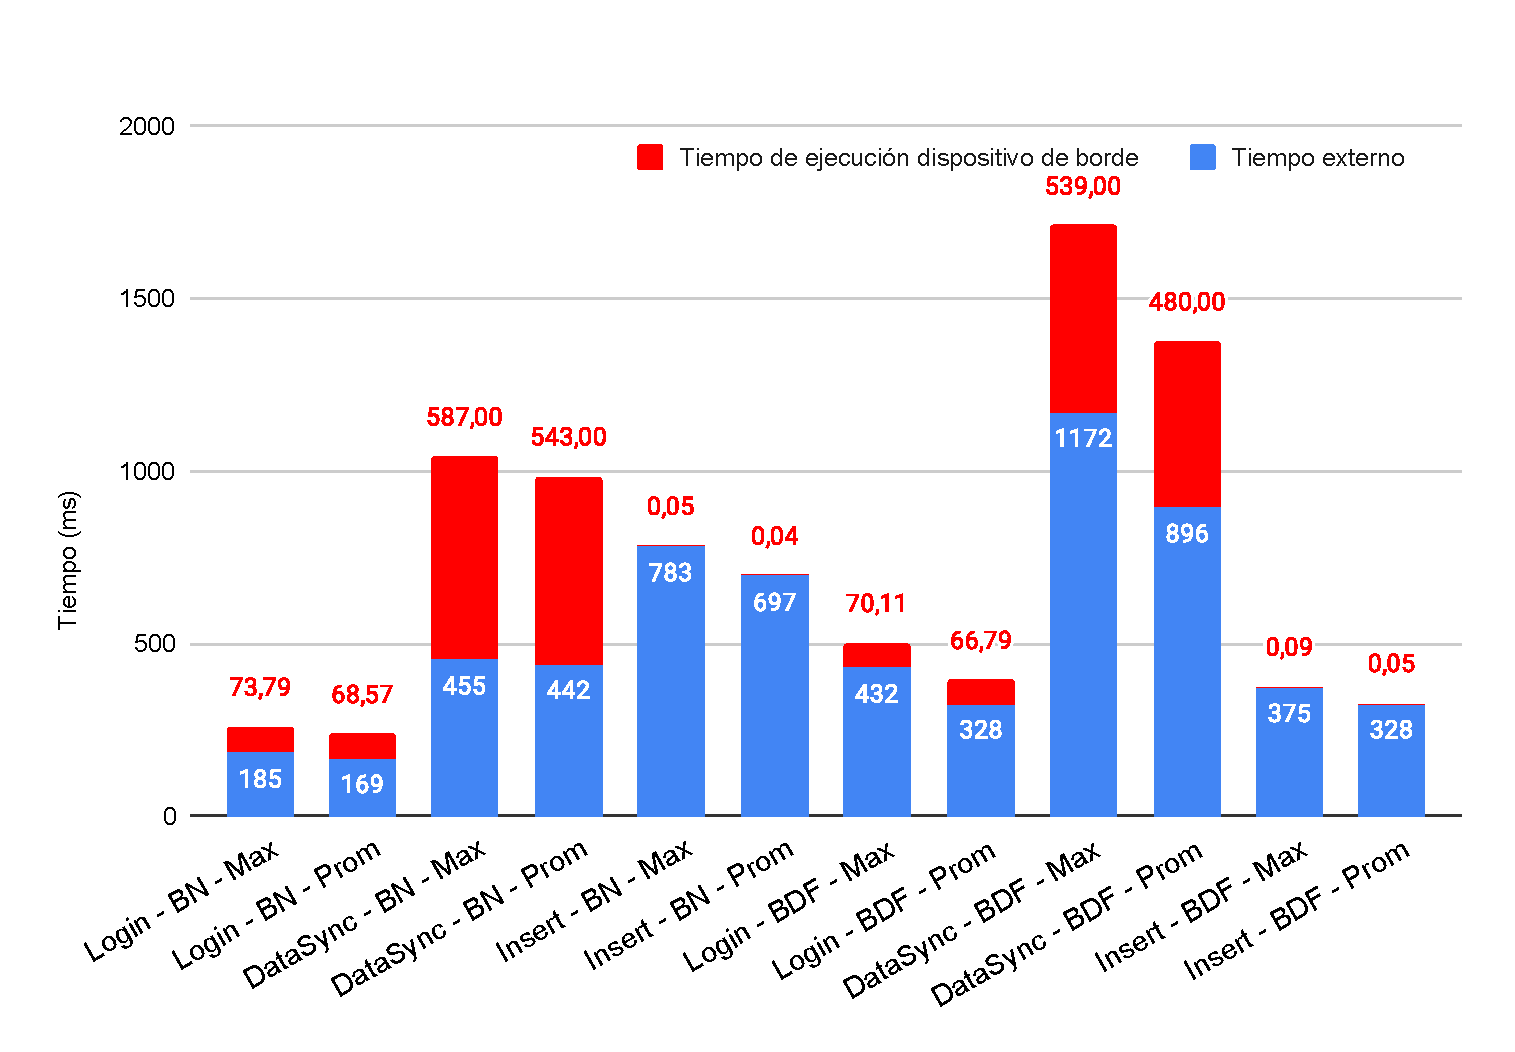
\includegraphics[width=\textwidth]{Imagenes/Experimentos/experimentoBarrasOperaciones.pdf}
        \caption{Evaluación inicial}
        \label{fig:evaluacionInicial}
\end{figure}

\section{Conectividad entre dispositivos}
\label{sec:conectividadDispositivos}
Con este experimento se busca someter a un dispositivo de niebla a una prueba de estrés ante múltiples conexiones y solicitudes concurrentes. Para ello se conectan hasta 64 dispositivos de borde de manera simultánea e incremental. Cada dispositivo de borde es emulado a través de un \textit{script} y se encuentra conectado a la misma red de área local que un dispositivo de niebla. Se simula una situación de pérdida de conectividad con la nube, por lo que no hay conexión con ella. Se realizan dos tipos de prueba diferentes:
\begin{itemize}
    \item \textbf{Prueba continua (PC):} Cada dispositivo de borde hace un \textit{insert}. Al hacerlo, como respuesta, recibe un mensaje de ``Ok'' y posteriormente un \textit{copy}, solo al recibir el \textit{copy}, un dispositivo de borde comienza a enviar otra solicitud de \textit{insert}.
    \item \textbf{Prueba periódica (PP):} Cada dispositivo de borde hace un \textit{insert} cada 30 segundos independientemente de si llega o no un \textit{copy}.
\end{itemize}

En ambos tipos de pruebas los tiempos medidos corresponden al intervalo entre el inicio de la operación de \textit{insert} y la recepción del \textit{copy} correspondiente. Durante todo el proceso, no se produjeron desconexiones ni se presentaron problemas relacionados con la red o con el dispositivo de niebla encargado de procesar la información.
 
El sistema se comportó correctamente en ambos tipos de pruebas. En la prueba continua (PC), se observó un tiempo promedio aproximado de 9570 ms para 64 dispositivos, 5140 ms para 32 dispositivos y 2280 ms para 16 dispositivos. También se realizaron pruebas con menos dispositivos, cuyos resultados se representan en la Figura \ref{fig:tiemposPromediosPruebas}. La diferencia en los tiempos es notable debido al crecimiento exponencial en la cantidad de mensajes de respuesta, lo que implica una mayor carga de cómputo sobre el dispositivo de niebla. Por ejemplo, si se utilizan 4 dispositivos de borde y cada uno realiza 4 \textit{inserts}, cada operación de \textit{insert} genera 4 operaciones de respuesta (\textit{copy}), lo que implica 16 mensajes de (\textit{copy}) en total, una para cada dispositivo de borde. Si se agregara otro dispositivo más, se tendría un total de 25 mensajes \textit{copy}.

En cuanto a los tiempos máximos en la prueba continua (PC), el sistema mantuvo un comportamiento adecuado y consistente a lo visto para los tiempos medios, registrando 12820 ms para 64 dispositivos, 5950 ms para 32 dispositivos y 2735 ms para 16 dispositivos, representados en la Figura \ref{fig:tiemposMaximosPruebas}.

En la prueba periódica (PP), se observó un tiempo medio de 5230 ms para 64 dispositivos, 2400 ms para 32 dispositivos y 1110 ms para 16 dispositivos. La diferencia de tiempos respecto a la prueba continua (PC) se debe a que el dispositivo de niebla tiene menos carga, esto se debe a que las operaciones \textit{insert} se realizan cada 30 segundos. En la Figura \ref{fig:tiemposPromediosPruebas} se muestra la comparativa de tiempos promedios para las diferentes cantidades de dispositivos.

En los tiempos máximos de la prueba periódica, el sistema también mostró un comportamiento adecuado y consistente, registrando 10775 ms para 64 dispositivos, 4715 ms para 32 dispositivos y 2140 ms para 16 dispositivos, como se muestra en la Figura \ref{fig:tiemposMaximosPruebas}.

\begin{figure}
    \centering
    \begin{minipage}{.8\textwidth}
        \centering
        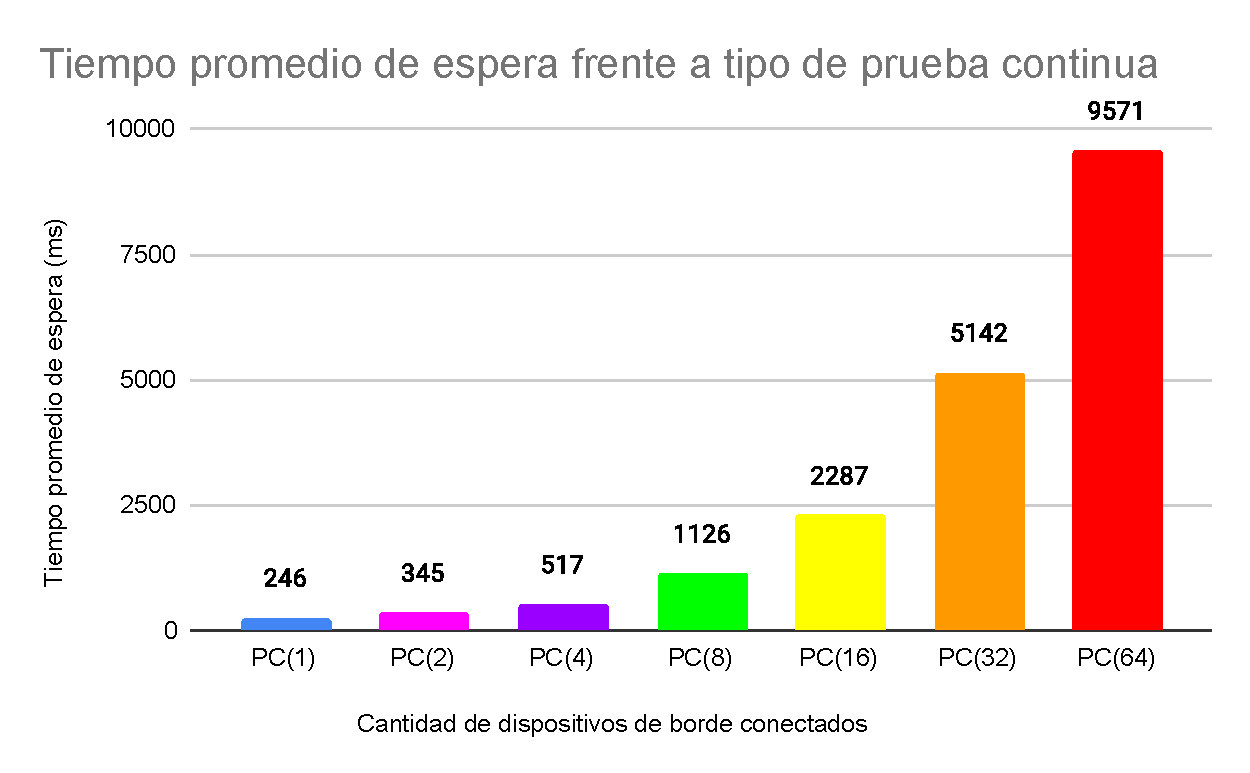
\includegraphics[width=\textwidth]{Imagenes/Experimentos/Tiempo promedio de espera frente a tipo de prueba continua.pdf}
    \end{minipage}%
    \hfill
    \begin{minipage}{.8\textwidth}
        \centering
        \includegraphics[width=\textwidth]{Imagenes/Experimentos/Tiempo promedio de espera frente a tipo de prueba periódica.pdf}
    \end{minipage}%
   
    \caption{Tiempos promedios de prueba continua y periódica}
    \label{fig:tiemposPromediosPruebas}
\end{figure}



\begin{figure}
    \centering
    \begin{minipage}{.8\textwidth}
        \centering
        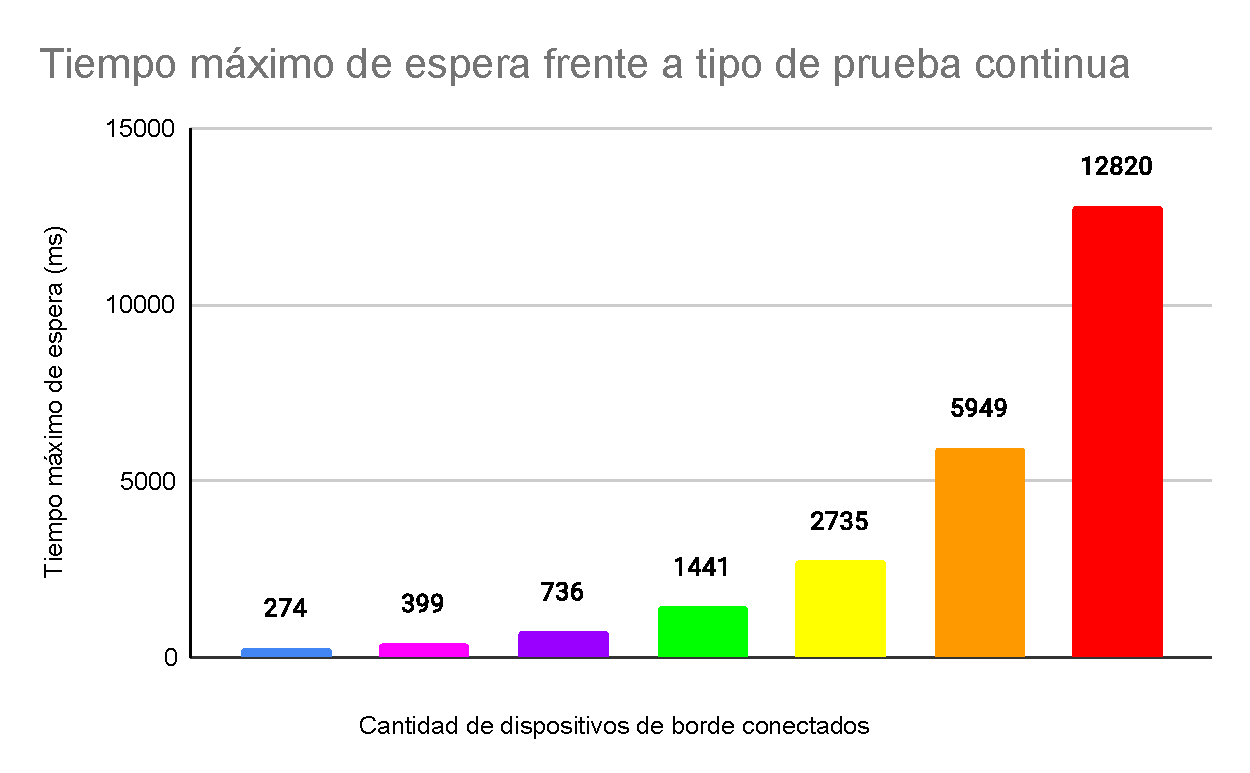
\includegraphics[width=\textwidth]{Imagenes/Experimentos/Tiempo maximo de espera frente a tipo de prueba continua.pdf}
    \end{minipage}%
    \hfill
    \begin{minipage}{.8\textwidth}
        \centering
        \includegraphics[width=\textwidth]{Imagenes/Experimentos/Tiempo maximo de espera frente a tipo de prueba periódica.pdf}
    \end{minipage}%
   
    \caption{Tiempos máximos de prueba continua y periódica}
    \label{fig:tiemposMaximosPruebas}
\end{figure}

A partir de los resultados observados y el análisis planteado se demuestra que la implementación del núcleo del sistema ALERTAR funciona exitosamente ante situaciones de alta carga con operaciones concurrentes sobre los dispositivos de niebla. Asegurando la consistencia y persistencia de los datos además de demostrar una alta capacidad de resiliencia ante eventos de falta de conectividad con servidores externos como lo es la nube.